%%%%%%%%%%%%%%%%%%%%%%%%%%%%%%%%%%%%%%%%%%%%%%%%%%%%%%%%%%%%%%%%%%%%%%%%
%    INSTITUTE OF PHYSICS PUBLISHING                                   %
%%%%%%%%%%%%%%%%%%%%%%%%%%%%%%%%%%%%%%%%%%%%%%%%%%%%%%%%%%%%%%%%%%%
%

\documentclass[10pt]{iopart}
\usepackage{siunitx}
\usepackage{units}
\usepackage[sort, compress]{cite}   
\usepackage{graphicx}   % Graphikpaket (fuer PNG,GIF,JPG)
\usepackage[pdfstartview=FitH,                     % Oeffnen mit fit width
                   breaklinks=true,                         % Umbrueche in Links, nur bei pdflatex default
                   bookmarksopen=true,                % aufgeklappte Bookmarks
                   bookmarksnumbered=true,        % Kapitelnummerierung in bookmarks
                   pdfprintscaling=None,                % Default-Einstellung zum Drucken: nicht skaliert
                   pdfduplex=DuplexFlipLongEdge, % Default-Druck-Einstellung: Duplex
					hidelinks,                   
                   ]{hyperref}

\newcommand{\gguide}{{\it Preparing graphics for IOP Publishing journals}}
%Uncomment next line if AMS fonts required
%\usepackage{iopams}  
\begin{document}

\title[Title on header]{Title in cover}

\author{Auuthors}

\address{Address}
\ead{email}
\vspace{10pt}
\begin{indented}
\item[]February 2014
\end{indented}

\begin{abstract}
Endoscopic methods play an increasingly important role in modern medicine. In general, the goal of endoscopy is to obtain as much information as possible for a viable diagnosis. To further improve diagnostics, there is a clear tendency towards multi-modal imaging by combining different imaging techniques. Making use of microscopy and Optical Coherence Tomography (OCT) in a single device is a promising approach to gather additional information and to thereby improve clinical diagnostics. 

The main goal of this work is the realization of a novel fiber scanner for 3D OCT imaging, designed for its combination with a full field microscope to form a multimodal probe. A tubular piezoelectric fiber scanner is used to perform en face scanning required for 3D OCT measurements. The complete scanning engine has an outer diameter of \SI{0.9}{\milli\meter} and a length of \SI{9}{\milli\meter}, and features custom fabricated \SI{10}{\micro\meter} thick polyimide flexible interconnect lines to address the four piezoelectric electrodes. To the best of our knowledge, the presented probe is one of the most compact implementation of an OCT microendoscope.

Optical and mechanical characterization of the scanner, implemented in a single modality demonstrator probe, show a high correlation with the analytical calculations and simulations. Thus, the approach described in this work constitutes a blueprint for a wide range of future scanning imaging probes.

\end{abstract}
% Uncomment for PACS numbers
%\pacs{00.00, 20.00, 42.10}
%
% Uncomment for keywords
%\vspace{2pc}
%\noindent{\it Keywords}: XXXXXX, YYYYYYYY, ZZZZZZZZZ
%
% Uncomment for Submitted to journal title message
%\submitto{\JPA}
%
% Uncomment if a separate title page is required
%\maketitle
% 
% For two-column output uncomment the next line and choose [10pt] rather than [12pt] in the \documentclass declaration
\ioptwocol
%

%%%%%%%%%%%%%%%%%%%%%%%%%%%%%%%%%%%%%%%%%%%%%%%%%%%%%%%%%%%%%%%%%%%%%%%%
\section{Introduction}
%%%%%%%%%%%%%%%%%%%%%%%%%%%%%%%%%%%%%%%%%%%%%%%%%%%%%%%%%%%%%%%%%%%%%%%%

%%%%%%%%%%%%%%%%%%%%%%%%%%%%%%%%%%%%%%%%%%%%%%%%%%%%%%%%%%%%%%%%%%%%%%%%
\section{Requirements of the scanner}
%%%%%%%%%%%%%%%%%%%%%%%%%%%%%%%%%%%%%%%%%%%%%%%%%%%%%%%%%%%%%%%%%%%%%%%%
\begin{figure}[h!]\centering 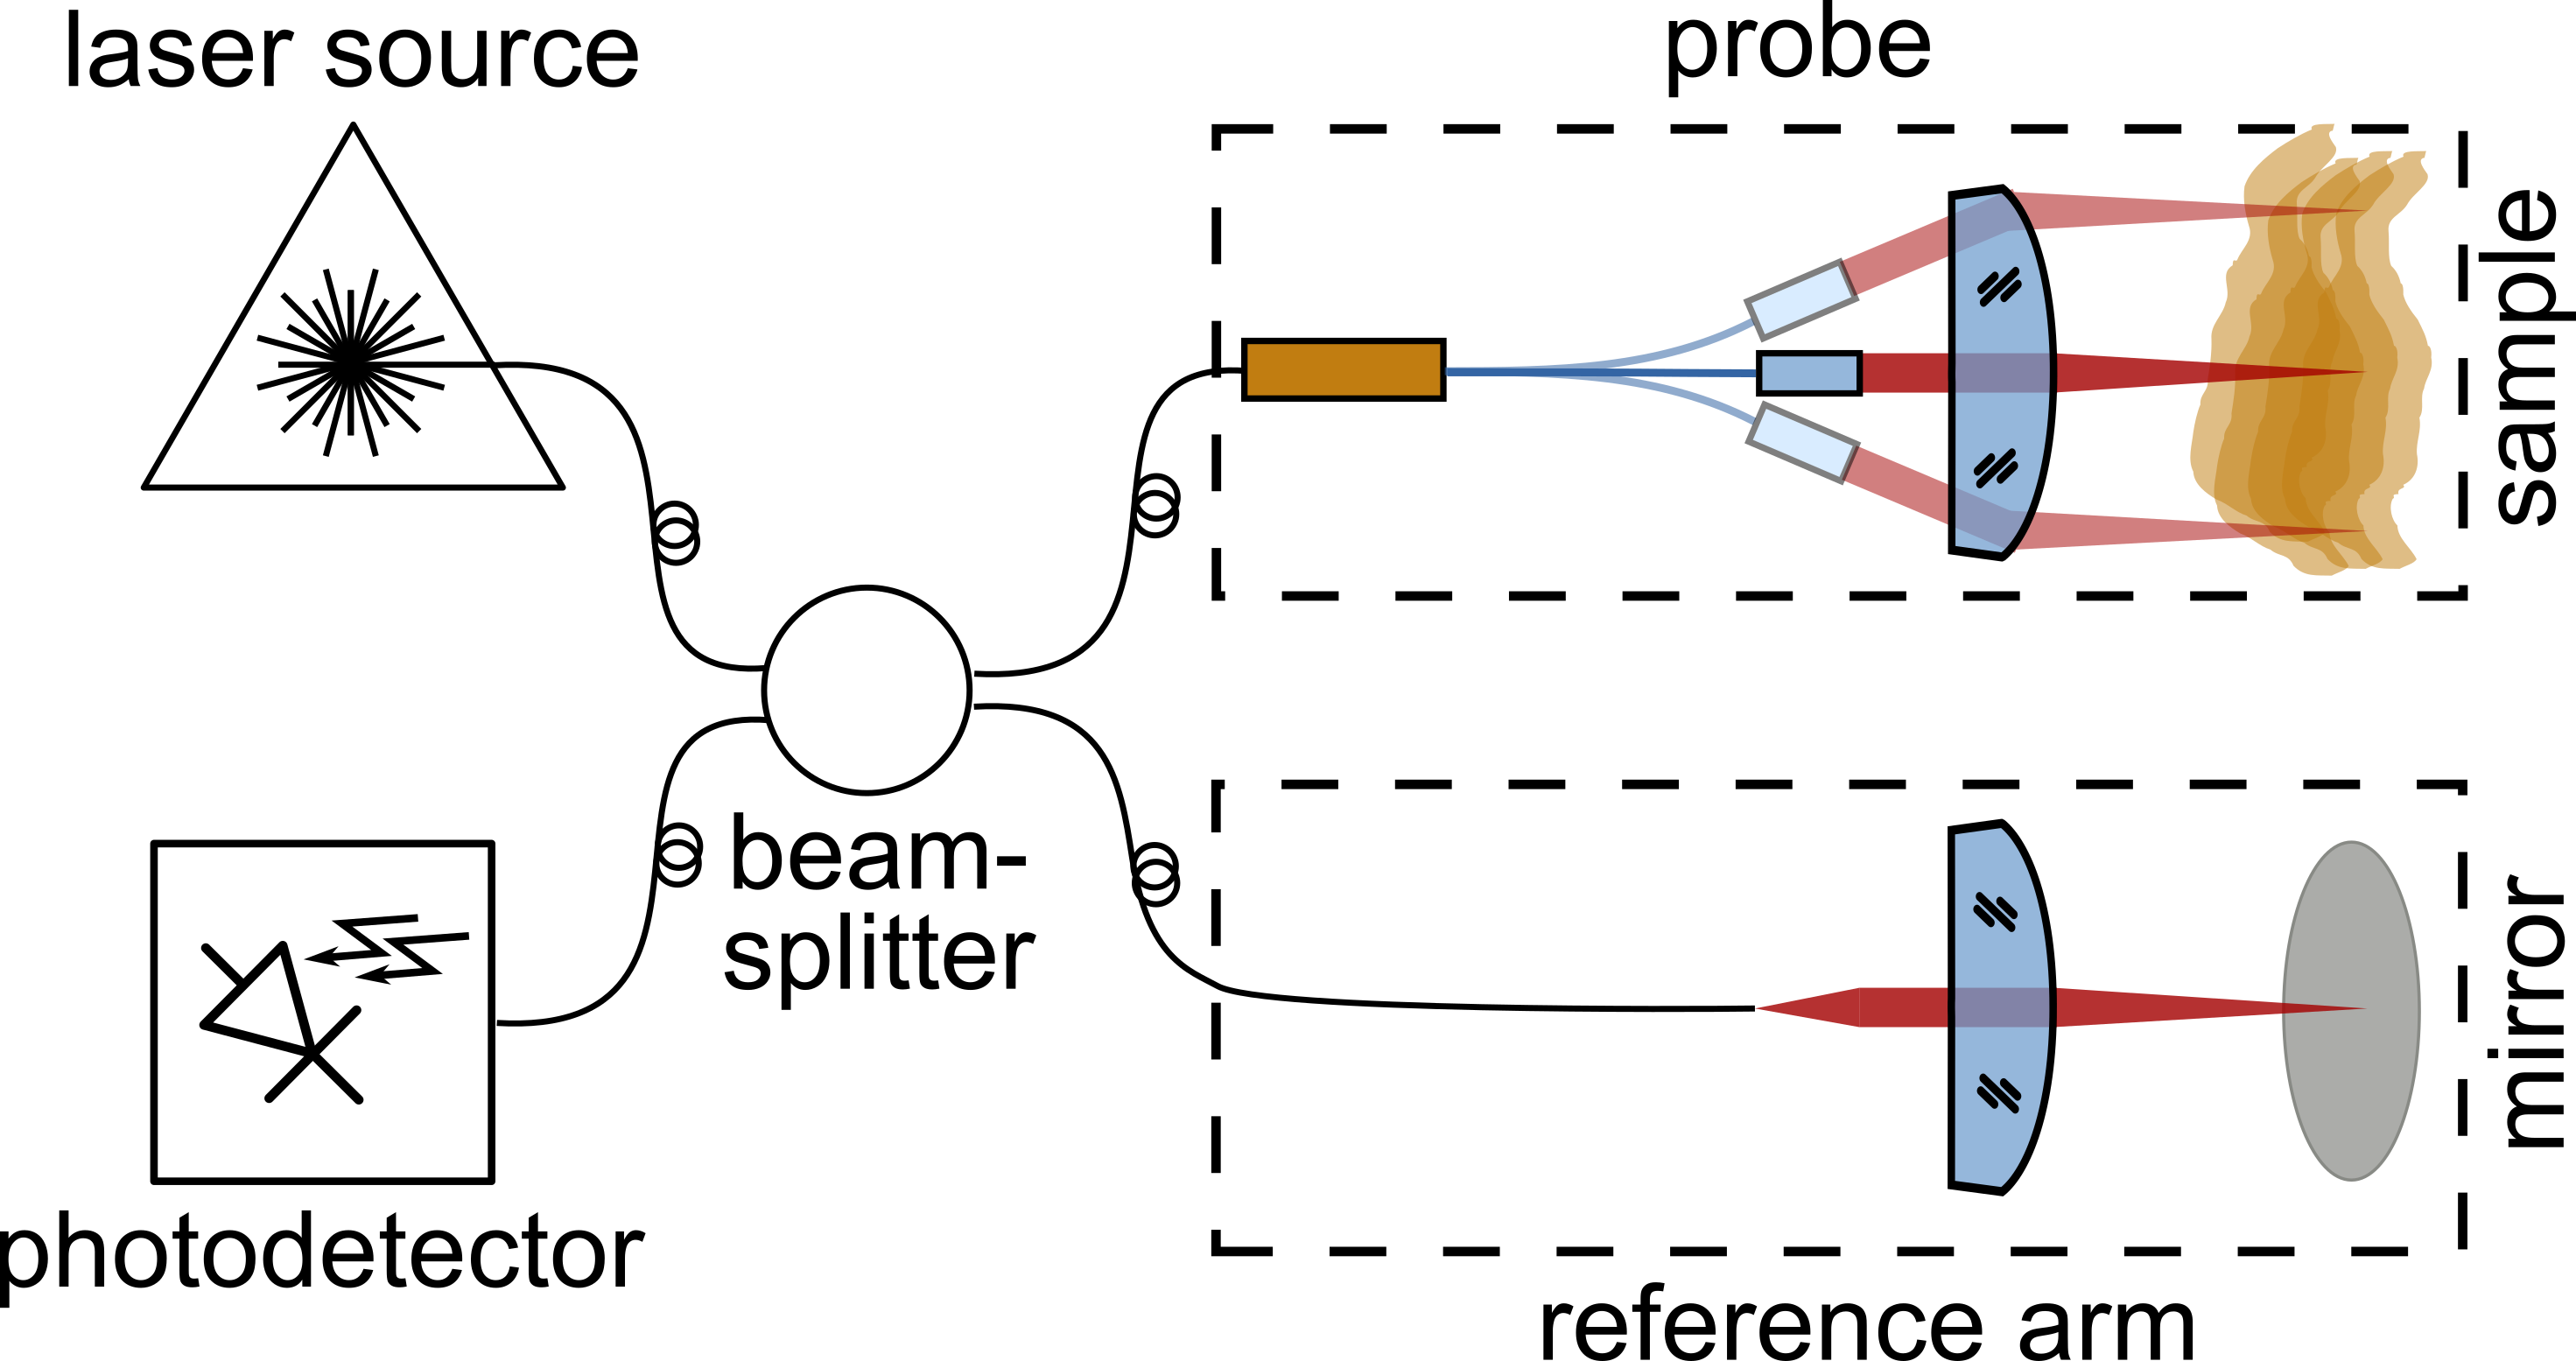
\includegraphics[width=\columnwidth]{figures/OCTsystem.png}
      \caption{OCT Requirements}
      %\label{}
\end{figure}

\paragraph{Optical requirements}

\begin{itemize}
\item A 2D scanning mechanism to enable 3D imaging.
\item The lateral resolution and depth of field should be adequate for OCT i.e. with numerical aperture ranging from 0.02 to 0.05.
\item The backreflections inside the probe should be minimized to reduce any loss of contrast and penetration depth.
\item The OCT field should be telecentric to avoid field curvature distortions.
\end{itemize}

\paragraph{Mechanical requirements}
\begin{itemize}
\item The field of view should be maximized for a 2 mm diameter objective lens that is shared with the endomicroscopy beam path.
\item The scanning speed should be adequate for the sampling rates characteristic of SS-OCT ($\sim \SI{100}{\kilo\hertz} $).
\item Its length should be minimized to allow its integration in flexible-head endoscopes.
\end{itemize}


%%%%%%%%%%%%%%%%%%%%%%%%%%%%%%%%%%%%%%%%%%%%%%%%%%%%%%%%%%%%%%%%%%%%%%%%
\section{Fourier plane scanner}
%%%%%%%%%%%%%%%%%%%%%%%%%%%%%%%%%%%%%%%%%%%%%%%%%%%%%%%%%%%%%%%%%%%%%%%%
As described in the previous section, the OCT optical setup samples the object at only a single point. Thus, the focus point has to be 2D-scanned over the surface of the sample to obtain 3D OCT images.

A very compact solution to achieve this are resonant fiber scanners. These devices use the concept of mechanical resonance to amplify the subtle movement of a piezoelectric actuator into a large displacement and angular deflection of the tip of a scanning fiber. 

The OCT beam path is designed as an distal-side telecentric system to avoid distortions in the 3D OCT measurement. To achieve this, the fiber scanner is driven with small angles and is positioned such that the lateral and angular movement of the scanner imitates the beam angles that can be observed in the collimated region of a classical telecentric lens system. Figure \ref{fig:fps} illustrates this approach. The whole scanner is buried in a channel with an inner diameter of \SI{1}{\milli\meter} limiting the movement of the scanner to a maximum angle $\theta$ of \SI{5}{\degree} that allows a maximum FOV of \SI{1}{\milli\meter} of the OCT beam path.

\begin{figure}[h!]\centering 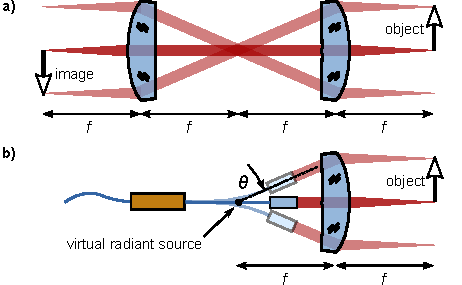
\includegraphics[width=6cm]{figures/fps2.pdf}
      \caption{\textbf{a)} Illustration of a classical telecentric system. The height of the object is translated into an angle $\theta$ in the collimated region between the two lenses. This angle is again translated into a corresponding image height by the second lens.
      \textbf{b)} Illustration of the OCT beam path using a fiber scanner in first resonance mode without micro prism and beamsplitter. The movement of the GRIN lens due to the fiber scanner and the distance between the GRIN lens and the focusing lens creating the same optical behavior as it can be observed in a classical distal-sided telecentric system. \textbf{c)} Nomenclature used in this work.}
      \label{fig:fps}		
\end{figure}



%%%%%%%%%%%%%%%%%%%%%%%%%%%%%%%%%%%%%%%%%%%%%%%%%%%%%%%%%%%%%%%%%%%%%%%%
\section{Mechanical design}
%%%%%%%%%%%%%%%%%%%%%%%%%%%%%%%%%%%%%%%%%%%%%%%%%%%%%%%%%%%%%%%%%%%%%%%%

The previous section focused in the acquisition of the depth information of a single column of a sample. But, in order to acquire a full, 3D volume of the sample, a 2D scanning mechanism is required. This section briefly goes over the physics and fundamental aspects of piezoelectric tube fiber scanners, starting with their actuation mechanism and followed by the analytical modeling of their resonant scanning fiber.

For the scanner to work as a Fourier plane scanner, at any point of the oscillation the output beam from the GRIN lens should point to a fixed virtual radiant source. This is fulfilled if the bending shape of the scanner is linear with the amplitude and thus, the ratio of the GRIN lens angle to its vertical displacement is kept constant $ y = d \cdot \tan \theta \simeq d \cdot \theta \Rightarrow \frac{\theta}{y} = const $ (refer to Figure \ref{fig:radiant}). According to simulations and experimental measurements, this is the case for this implementation.

\begin{figure}[h!]\centering
      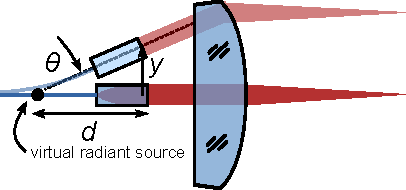
\includegraphics[width=5cm]{figures/radiant.pdf}
      \caption{Schematic of the Fourier plane scanner at rest and at an arbitrary angle $\theta$. If the scanner behaves linearly, the output beam will appear to come from a fixed virtual radiant source regardless of the scanning amplitude.}
      \label{fig:radiant}
\end{figure}

\begin{figure}[h!]\centering 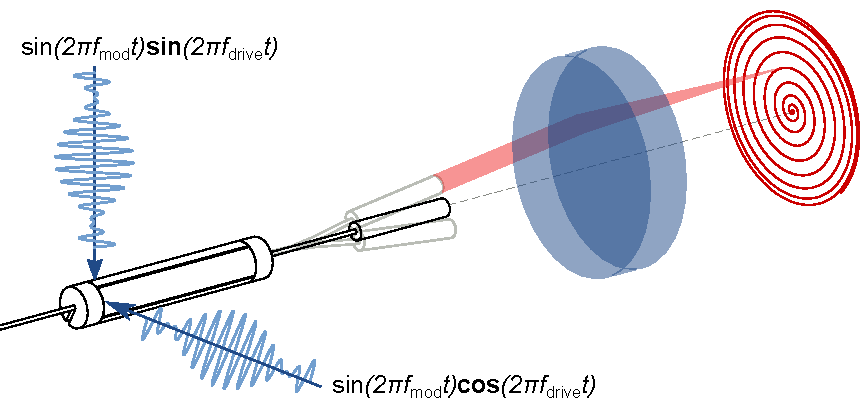
\includegraphics[width=\columnwidth]{figures/PZTDrivingMoving.pdf}
      \caption{Schematic of the piezoelectric tube, fiber, GRIN and objective lens focusing the OCT beam (red) in a plane. 
      The piezoelectric tube is driven with two independent amplitude modulated sine and cosine signals to generate a spiral pattern, used to acquire an image. }
      \label{fig:PZTDriving}
\end{figure}

As explained in the previous section, in any resonant system, its geometrical and mechanical characteristics fully define the operating frequency range, and with it, constrain the way the final image can be sampled.

In the following paragraphs the behavior of the fiber scanner is mechanically modeled, and this information used to choose the most relevant fabrication parameters leading to an adequate resonant frequency for OCT.

\subsection{Piezoelectric tube actuators}
\label{ssec:piezo}
A piezoelectric tube is a solid state actuator consisting of a tube made of radially polarized piezoelectric material with one inner and four outer electrodes, as depicted in \autoref{fig:pztTheory}a. 
\begin{figure}[h!]
      \centering
      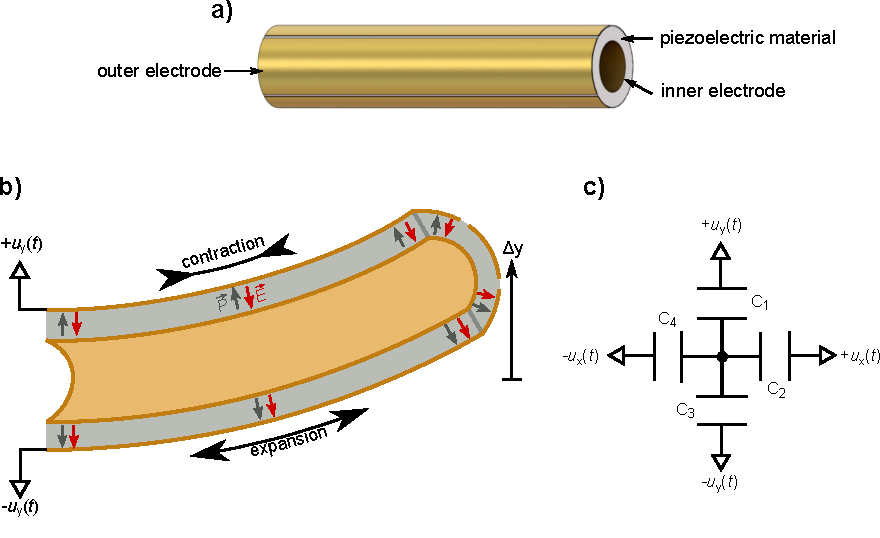
\includegraphics[width=\columnwidth]{figures/pztTheory.pdf}
      \caption{	\textbf{a)} Render of a piezoelectric tube.
      			\textbf{b)} Half-cut drawing of a piezoelectric tube in actuated state. The radial polarization of the piezoelectric material is shown in gray arrows. A voltage $\pm u_\mathrm{y}(t)$ is applied to the top and bottom outer electrodes, creating a radial electric field under those electrodes, depicted as red arrows. Due to the piezoelectric effect, the top quarter of the tube contracts, while the bottom quarter expands, inducing a bending of the tube and a deflection of its tip $\Delta y(V)$.
      			\textbf{c)} Electrical model of the piezoelectric tube with four electrodes.}
      \label{fig:pztTheory}
\end{figure}
The outer metallization of the tube is divided in four quarter electrodes, which generate a radial electric field in the sandwiched portion of the piezoelectric material, shown in \autoref{fig:pztTheory}b. If a voltage difference is applied to two opposite electrodes of the tube, one side will contract while the other will expand due to the piezoelectric effect. This behavior is modeled linearly  as $\epsilon = d_{31} E$ \cite{Arnau2008}, where $\epsilon$ represents the in-plane strain, $d_{31}$ the piezoelectric strain coefficient, and \textit{E} the out-of-plane electric field magnitude. This asymmetry creates a bending moment across the axis of the tube, inducing its deformation. If one end of the actuator is kept static, the tip of the actuator will deflect and tilt according to the applied voltage. A 2D scanner can be created out of this setup if two independent signals control the horizontal and vertical electrodes, as shown in \autoref{fig:pztTheory}c.

The deflection of the tip of the tube reacts linearly with the applied voltage, and in case of bipolar operation, estimated by \cite{Chen} as

\begin{equation}
\Delta y = V  \frac{2 \sqrt{2} d_{31} L^2}{\pi D h},
\end{equation}

where \textit{V} is the voltage applied to each opposing electrode, $d_{31}$ is the piezoelectric strain coefficient of the material in direction perpendicular to the polarization direction, \textit{L} is the length of the tube, \textit{D} its outer diameter and \textit{h} the thickness of its wall. Thus, longer tubes with a thinner diameter and wall thickness maximize the deflection of the tip. Typical deflections for small actuators lie in the order of $\SI{20}{\nano\meter / \volt}$.


\subsection{Resonant beam theory}
\label{sec:EB}
The piezoelectric actuator described in the last paragraphs couples mechanical energy into the cantilever of the scanner, formed by a optical fiber segment to which a GRIN lens is glued, as depicted in \autoref{fig:EBth}a. As the scanner uses mechanical resonance to amplify the small displacements of the actuator, it is important to analyze the resonance frequency of such a system. 

\begin{figure}[h!]\centering
      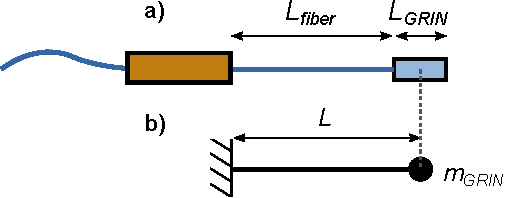
\includegraphics[width=6cm]{figures/EB.pdf}
      \caption{\textbf{a)} Schematic drawing of the piezoelectric scanner, composed of a piezoelectric tube, fiber and GRIN lens. 
      \textbf{b)} Simplified mechanical diagram obtained by modeling the fiber as a weightless cantilever and the GRIN lens as a point mass.}
      \label{fig:EB}
\end{figure}

The fiber-GRIN assembly can be modeled as a point-loaded, fixed-free cantilever where the weight of the GRIN lens is concentrated in its center of gravity, as represented in Figure \ref{fig:EBth}b. 

Now, by applying the ideal mass-spring harmonic resonator equation, the resonance frequency can be estimated as 
\begin{equation}
f_\mathrm{res} = \frac{1}{2 \pi} \sqrt{\frac{K_\mathrm{cantilever}}{m_{\mathrm{GRIN}}}} 
\label{eq:fres}
\end{equation}
where $K_\mathrm{cantilever}$ represents the elastic constant of the fiber cantilever. Considering it as a fixed-free, point loaded cantilever, its spring constant can be calculated as 
\begin{equation}
K_\mathrm{cantilever} = \frac{3 E I}{L^3} = \frac{3 \pi}{4} \frac{E_\mathrm{fiber} r_\mathrm{fiber}^4}{L^3}
\label{eq:EB}
\end{equation}
following the Euler-Bernoulli theory \cite{MarcJ.Madou2011} and considering that the moment of inertia of the cylindrical fiber is given by $I_\mathrm{fiber} = \frac{\pi}{4} r^4$. 

\subsection{Resonance frequency calculation}
The scanner used in the probe consists of a piezoelectric tube which drives a beam composed of a single mode fiber and a GRIN lens into resonance, as depicted in \autoref{fig:EB}a.  



The Euler-Bernoulli method can be used to estimate the resonant frequency of this scanner as detailed in \autoref{sec:EB}. The resulting equations \ref{eq:fres} and \ref{eq:EB} show how the different mechanical properties of the scanner influence its resonant frequency. Thus, this frequency can be reduced in different ways: increasing the cantilever length $L$, decreasing the radius of the fiber $r_\mathrm{fiber}$ or increasing the mass at the tip $m_{\mathrm{GRIN}}$. First, by having a GRIN lens attached at the tip, the resonance frequency is reduced by a factor of 62\%. Furthermore, by choosing a fiber with a cladding diameter of \SI{80}{\micro\meter} instead of the standard \SI{125}{\micro\meter}, the resonance frequency can be lowered by an extra factor of 60\%, as the sensitivity of the resonance frequency to the diameter of the fiber is quadratic. Under these conditions, the resonant frequency vs. length of the cantilever formed by a \SI{80}{\micro\meter} fused silica fiber with the chosen GRIN lens is computed in Figure \ref{fig:freq} using Equations \ref{eq:fres} and \ref{eq:EB}.

When selecting the length of the scanner, there are two details to consider. First, as the scanner is buried in a \SI{1}{\milli\meter} channel, the maximum displacement of the \SI{350}{\micro\meter} GRIN lens is limited to $\pm\SI{325}{\micro\meter}$. Within that small displacement we want to achieve the maximum angular deflection of the GRIN lens to maximize the FOV. This can be achieved by using shorter fiber lengths, which induces a smaller radius of curvature. This shows a trade-off with the density of sampling $N_\mathrm{T}$, which is increased with longer fiber lengths. To balance those terms, we chose a total scanner length of \SI{4.5}{\milli\meter}, which fulfills all the before-mentioned requirements, as \autoref{tab:mech} shows. 

\begin{table}[h!]\centering
	\caption{Mechanical characteristics of the fiber scanner at its designed working point.}
	\begin{tabular}{rl}\\
		\hline
		\textbf{Cantilever length} & \SI{4.5}{\milli\meter} \\ 
		\textbf{Resonant Frequency} & \SI{770}{\hertz} \\ 
		\textbf{Max. angular deflection} & \SI{5}{\degree} \\ 
		\hline
	\end{tabular} 
    \label{tab:mech}
\end{table}

\subsection{COMSOL simulation}

In order to validate the theoretical analysis of the previous section, a multiphysics finite element analysis was performed using \textit{COMSOL}. The actuator was modeled as a radially polarized piezoelectric material (\textit{PIC 151}) and the rest of the structure as fused silica. The excitation voltage is a sinusoidal symmetrical potential between the top and bottom electrodes of the tube. Note that, as the system undergoes small deflections, it is simulated assuming linear behavior without incurring in important deviations \cite{Fertis2006}.

As the first step, the resonant frequency of the system is simulated. An \textit{Eigenfrequency} study calculate the first mode resonance at \SI{762}{\hertz}, which closely matches the analytical estimation of \SI{770}{\hertz}. The mode shape at resonance is shown in Figure \ref{fig:defle}, where it can be observed that the actuator and the base of the fiber are almost static, confirming the resonant behavior of the scanner.

\begin{figure}[h!]\centering
      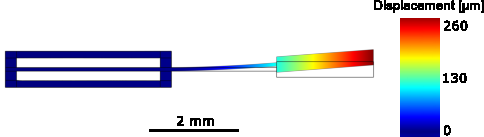
\includegraphics[width=\columnwidth]{figures/deflection.pdf}
      \caption{COMSOL simulation showing a cross section of the scanner maximum deflection at resonance for an actuation voltage of $\pm \SI{75}{\volt}$. The deformed structure is color coded showing the total displacement from the rest position (shown outlined). }
      \label{fig:defle}
\end{figure}

%Note that, as the system is working at its resonance, it is very difficult to simulate the oscillation amplitude, as it depends on its damping factor which should be obtained experimentally. Thus, for the simulation, this value was chosen to fit the expected deflection. 

Thanks to the multiphysics simulation, it is also possible to check the electric field distribution inside the piezoelectric tube. As can be seen in Figure \ref{fig:field}, for a symmetrical actuation in the top and bottom electrodes with a voltage of $\pm \SI{75}{\volt}$, most of the volume under these electrodes experiences a field magnitude close to the expected theoretical value 
\begin{equation}
E= \frac{U}{d}  = \frac{\SI{75}{\volt}}{\SI{150}{\micro\meter}}  = \SI{500}{\volt/\meter},
\end{equation}
which is under the safe operating field of \textit{PIC 151}, which ranges from $ +\SI{1000}{\volt/\meter}$ to $ -\SI{700}{\volt/\meter}$. Only some fringe areas exceed these values, which could become depolarized with time.
\begin{figure}[h!]\centering
      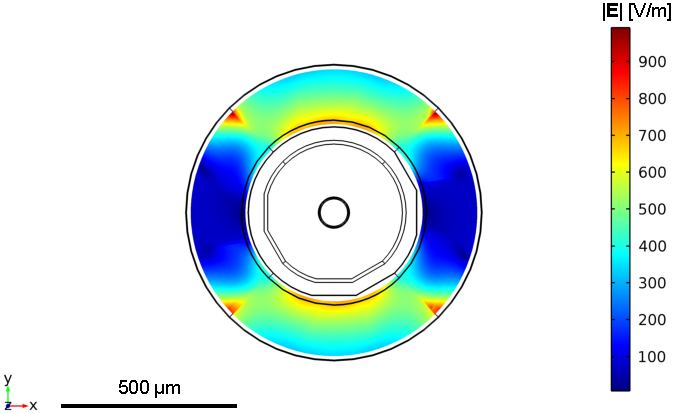
\includegraphics[width=\columnwidth]{figures/field.pdf}
      \caption{Magnitude of the electrical field inside a cross-section of the piezoelectric tube with an excitation voltage of $\pm \SI{75}{\volt}$ applied to the top and bottom electrodes.}.
      \label{fig:field}
\end{figure}


%%%%%%%%%%%%%%%%%%%%%%%%%%%%%%%%%%%%%%%%%%%%%%%%%%%%%%%%%%%%%%%%%%%%%%%%
\section{Optical design}
%%%%%%%%%%%%%%%%%%%%%%%%%%%%%%%%%%%%%%%%%%%%%%%%%%%%%%%%%%%%%%%%%%%%%%%%


In a Fourier plane scanner, the numerical apertures and focal lengths of the scanning and objective lens are related by the diameter of the beam in the intermediate region between both lenses. Thus, based on the schematic of Figure \ref{fig:fps}c, the following geometrical optics relations are obtained: $d_\mathrm{beam} \simeq 2\cdot f_\mathrm{GRIN}\cdot \mathrm{NA}_\mathrm{fiber}$ and $d_\mathrm{beam} \simeq 2 \cdot f_\mathrm{obj}\cdot \mathrm{NA}_\mathrm{OCT}$. By combining them together,

\begin{equation}
f_\mathrm{GRIN} \cdot \mathrm{NA}_\mathrm{fiber} = f_\mathrm{obj} \cdot \mathrm{NA}_\mathrm{OCT}
\label{eq:fpsNA}
\end{equation}

the main design equation for the scanner is obtained. Note that these equations use a small angle approximation valid for small NA:  $\tan[\sin^{-1}(\mathrm{NA})] \simeq \mathrm{NA} $. In this case, as any NA is smaller than 0.25, the error of this simplification is smaller than 2\%.


\subsubsection{Resolution of LSI and confocal systems}

The autocorrelation of the MTF which characterizes LSI and confocal microscopy can lead to an increase in resolution compared with conventional microscopy if the illumination source and an detection aperture are significantly smaller than the diffraction limited PSF in these surfaces. In this situation $PSF_{\rm{core}}$ becomes a delta function . 

In this work, the pinhole is defined by the diameter of the GRIN lens, which truncates the collimated beam at its $1/e^2$ level, corresponding with a truncation factor $K=1$. This limits the resolution of the system compared with a fully confocal system, where $K\rightarrow \infty$, as seen in \ref{fig:fullPartialConfocal}.

\begin{figure}[h!]\centering 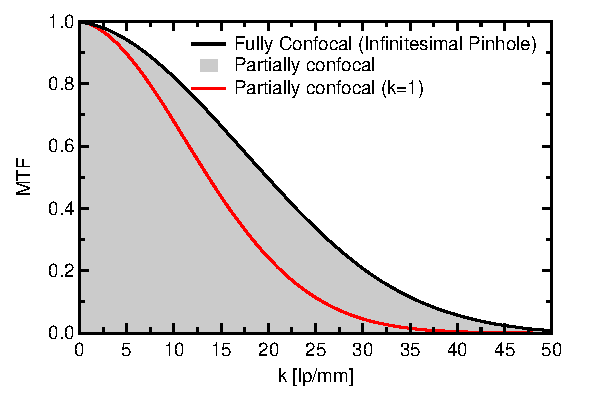
\includegraphics[width=\columnwidth]{figures/fullPartialConfocal.pdf}
      \caption{	Comparison of the simulated MTF of a confocal system with infinitesimally small pinhole (black) and with a pinhole with a truncation factor $K=1$ (red), as used in this work. The shaded area represents the possible MTFs locus for any truncation factor.}
      \label{fig:fullPartialConfocal}
\end{figure}

As stated in \autoref{sec:designov}, in order to independently test the behavior of the OCT scanner and optics, a single modality probe was fabricated as a demonstrator. Its optical design, depicted in \autoref{fig:single}, emulates the multimodal design from \autoref{fig:BS} by unfolding its optical path. The main difference is the lack of the prism and beamsplitter and the orientation of the planoconvex lens, which is flipped to reduce the backreflections caused by normal incidence on the planar side of the lens.


\begin{figure}[h!]\centering
      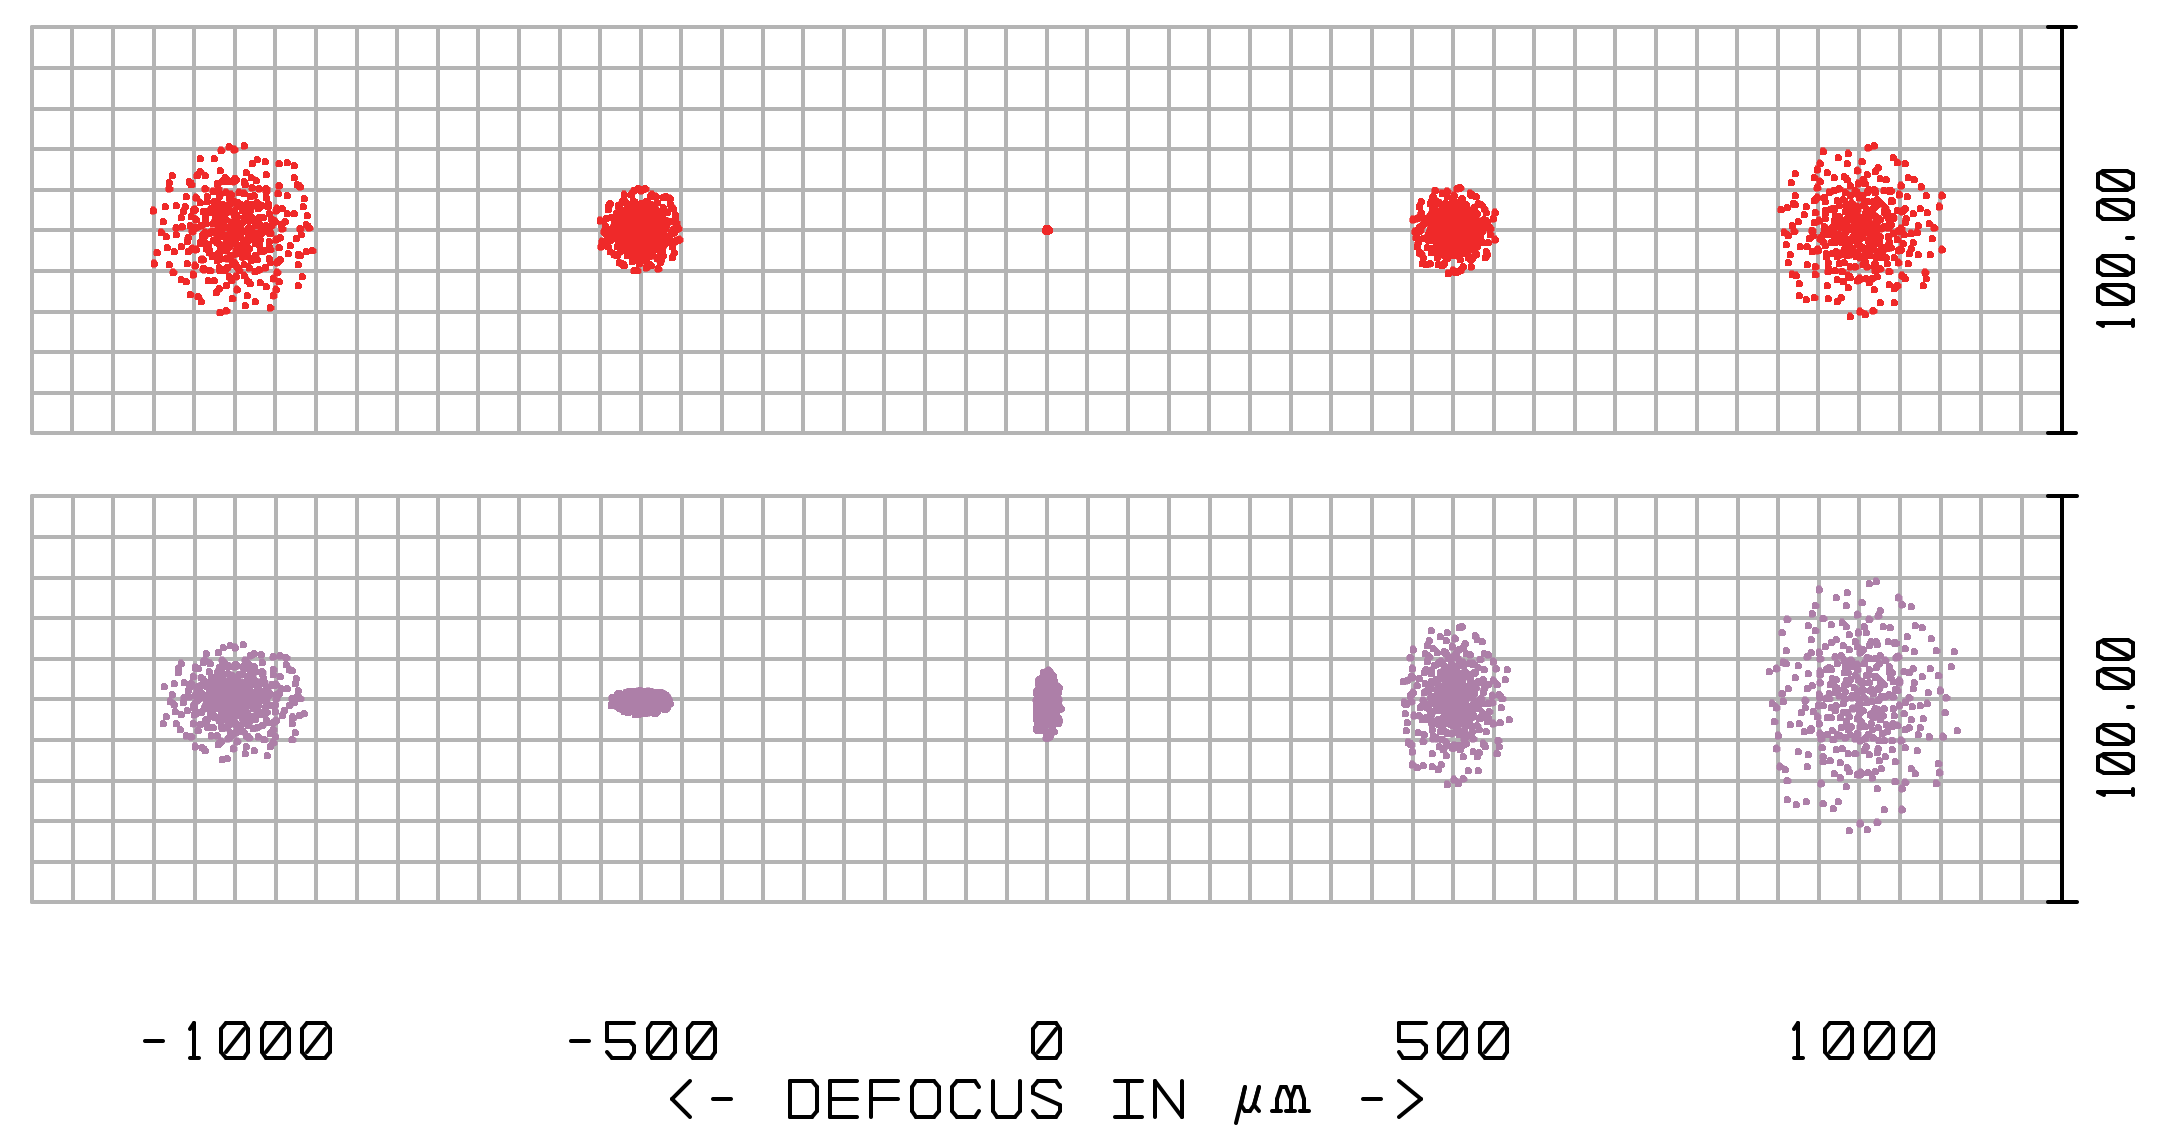
\includegraphics[width=\columnwidth]{figures/singleSpot.png}
      \caption{Simulated spot through focus}
      \label{fig:MTFcomp}
\end{figure}

%%%%%%%%%%%%%%%%%%%%%%%%%%%%%%%%%%%%%%%%%%%%%%%%%%%%%%%%%%%%%%%%%%%%%%%%
\section{Spiral Scanning}
%%%%%%%%%%%%%%%%%%%%%%%%%%%%%%%%%%%%%%%%%%%%%%%%%%%%%%%%%%%%%%%%%%%%%%%%


As described in the previous section, the OCT optical setup samples the object at only a single point. Thus, the focus point has to be 2D-scanned over the surface of the sample to obtain 3D OCT images.

A very compact solution to achieve this are resonant fiber scanners. These devices use the concept of mechanical resonance to amplify the subtle movement of a piezoelectric actuator into a large displacement and angular deflection of the tip of a scanning fiber. 

As any resonant system, the movement of the scanning fiber is constrained to harmonic oscillations within a frequency close to its resonance frequency $f_\mathrm{res}$. This requirement limits the possible scanning patters to harmonic movements at $f_\mathrm{res}$, excluding then raster scanning, which require at least an axis working out of resonance. Then, conventional alternatives are Lissajous \cite{Moon2010} and spiral scanning. In order to ease the reconstruction of the image, this work implements the latter.

The following pages describe the concept of spiral scanning, its characteristics, limitations and implementation.

%%*****************************************************************************
\subsection*{Driving and acquisition}
%%*****************************************************************************
The piezoelectric tube which drives the scanner has four outer gold electrodes to control the lateral movement of the scanner, as described in \autoref{ssec:piezo}. Two independent voltage sources control the vertical and horizontal movement of the actuator by addressing the corresponding pair of electrodes. If sine and cosine signals of the same frequency $f_\mathrm{drive}$ are used to drive the scanner, the GRIN lens will oscillate in a circle of constant radius. If now the amplitude of these signals is amplitude modulated with another sinusoidal signal of frequency $f_\mathrm{mod}$, the resultant trajectory will be spiral, as illustrated in \autoref{fig:PZTDriving}.

\begin{figure}[h!]\centering 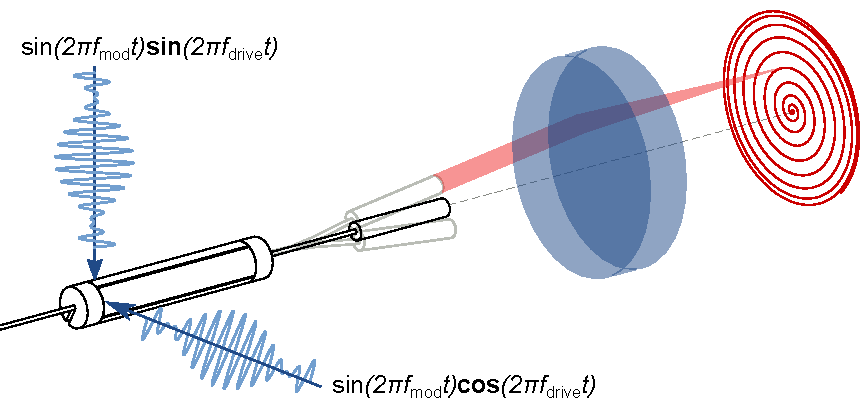
\includegraphics[width=\columnwidth]{figures/PZTDrivingMoving.pdf}
      \caption{Schematic of the piezoelectric tube, fiber, GRIN and objective lens focusing the OCT beam (red) in a plane. 
      The piezoelectric tube is driven with two independent amplitude modulated sine and cosine signals to generate a spiral pattern, used to acquire an image. }
      \label{fig:PZTDriving}
\end{figure}

During the full period of the spiral pattern $T_\mathrm{spiral}=f_\mathrm{mod}^{-1}$ , two complete frames are acquired, one while the spiral grows, another while it shrinks. The whole pattern can be divided in $N_\mathrm{rings} = f_\mathrm{drive}/f_\mathrm{mod}$ individual rings, as depicted in \autoref{fig:spiralScanningNT}, each one acquired in a period $T_\mathrm{ring}=f_\mathrm{drive}^{-1}$. Thus the number of sample points that can be acquired in an individual ring
\begin{figure}[h!]\centering
      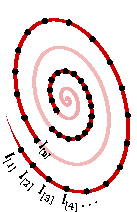
\includegraphics[width=3cm]{figures/spiralScanningNT.pdf}
      \caption{Section of a spiral trajectory highlighting two different rings. The $n$ black dots represent the sampling points of each ring. Notice that in the inner ring the sampling density is higher than in the outer one.}
      \label{fig:spiralScanningNT}
\end{figure}
\begin{equation}
n = \frac{f_\mathrm{s}}{f_\mathrm{drive}}
\label{eq:nT}
\end{equation}
depends only on the driving frequency of the scanner $f_\mathrm{drive}$ and the sampling frequency $f_\mathrm{s}$ of the spectrometer, which is usually constant. This value is very important, as it defines the spatial sampling density. 

In order to fulfill the Nyquist theorem, the spacing between two adjacent sample points should be smaller than the Airy radius of the laser spot. This condition is easily fulfilled in the inner rings of the spiral, where the focus spot moves at low speed. But as the radius of the spiral grows, so does the scanning speed and therefore the distance between sample points, as seen in \autoref{fig:spiralScanningNT}.

It is clear then that spiral scanning shows a non-uniform sampling distribution across the imaging field, which is confirmed experimentally in \autoref{fig:calib}. Thus, to avoid undersampling in the outer areas, the number of samples per ring $n$ should be as high as possible. As OCT systems have a relatively small sampling frequency ($\sim$\SI{100}{\kilo\hertz}), the resonant frequency needs to be below \SI{1}{kHz} to achieve more than 100 acquired points per ring of the spiral.



%%%%%%%%%%%%%%%%%%%%%%%%%%%%%%%%%%%%%%%%%%%%%%%%%%%%%%%%%%%%%%%%%%%%%%%%
\section{Fabrication and assembly}
%%%%%%%%%%%%%%%%%%%%%%%%%%%%%%%%%%%%%%%%%%%%%%%%%%%%%%%%%%%%%%%%%%%%%%%%


This chapter details the implementation of the probe shown in \autoref{fig:overview}, which serves as a demonstrator of the fiber scanner design and evaluation tool of the optical performance of the OCT beam path.

\begin{figure}[h!]\centering 
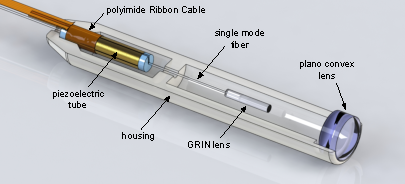
\includegraphics[width=\columnwidth]{figures/overview.pdf}
      \caption{CAD of the single modality demonstrator with the top of the housing removed. Total length: \SI{15}{\milli\meter}.}
      \label{fig:overview}
\end{figure}

The design can be summarized as follows: The piezoelectric actuator has four outer gold electrodes to control the lateral movement of the scanner. The addressing of these electrodes is realized by a ribbon cable, which is wrapped around the piezoelectric tube. The single mode fiber is centered in the piezoelectric tube and the GRIN lens bonded to the tip of this fiber. This arrangement enables a compact fiber scanner with a total length of \SI{9}{\milli\meter} and a resonance frequency of \SI{750}{\hertz} optimized for an OCT system with an A-Scan repetition rate of \SI{100}{\kilo\hertz}.

The following paragraphs describe the manufacturing process and assembly of the most relevant components of the probe, beginning with the fabrication of the polyimide electrodes used for contacting the piezoelectric tube and proceeding with details of the necessary assembly steps to fabricate the scanner, leading to the assembly of the complete probe.

\subsection{Polyimide electrodes}

The first challenge that appears in the manufacturing of the scanner lies in contacting the four external electrodes of the piezoelectric tube. 

Due to the small diameter of the tube (\SI{800}{\micro\meter}), creating a reliable interface between the driving circuit and its electrodes is not trivial. Other piezoscanner implementations use soft soldering and insulated copper wires \cite{Lee2010, Meinert, Huo2010}, but the soldering process can damage the piezoelectric material, as it is exposed to temperatures above its Curie temperature. This method also increases the diameter of the actuator significantly, as a solder blob is needed. %Furthermore, it requires welding by hand in a \SI{600}{\micro\meter} curved electrode.

Instead, this design uses a polyimide ribbon cable which is wrapped around the piezotube and addresses its four external electrodes using vias. Its geometry, cross section and application over the tube is depicted in Figure \ref{fig:piRolled}, while \autoref{fig:piRender} shows its complete design.

\begin{figure}[h!]\centering 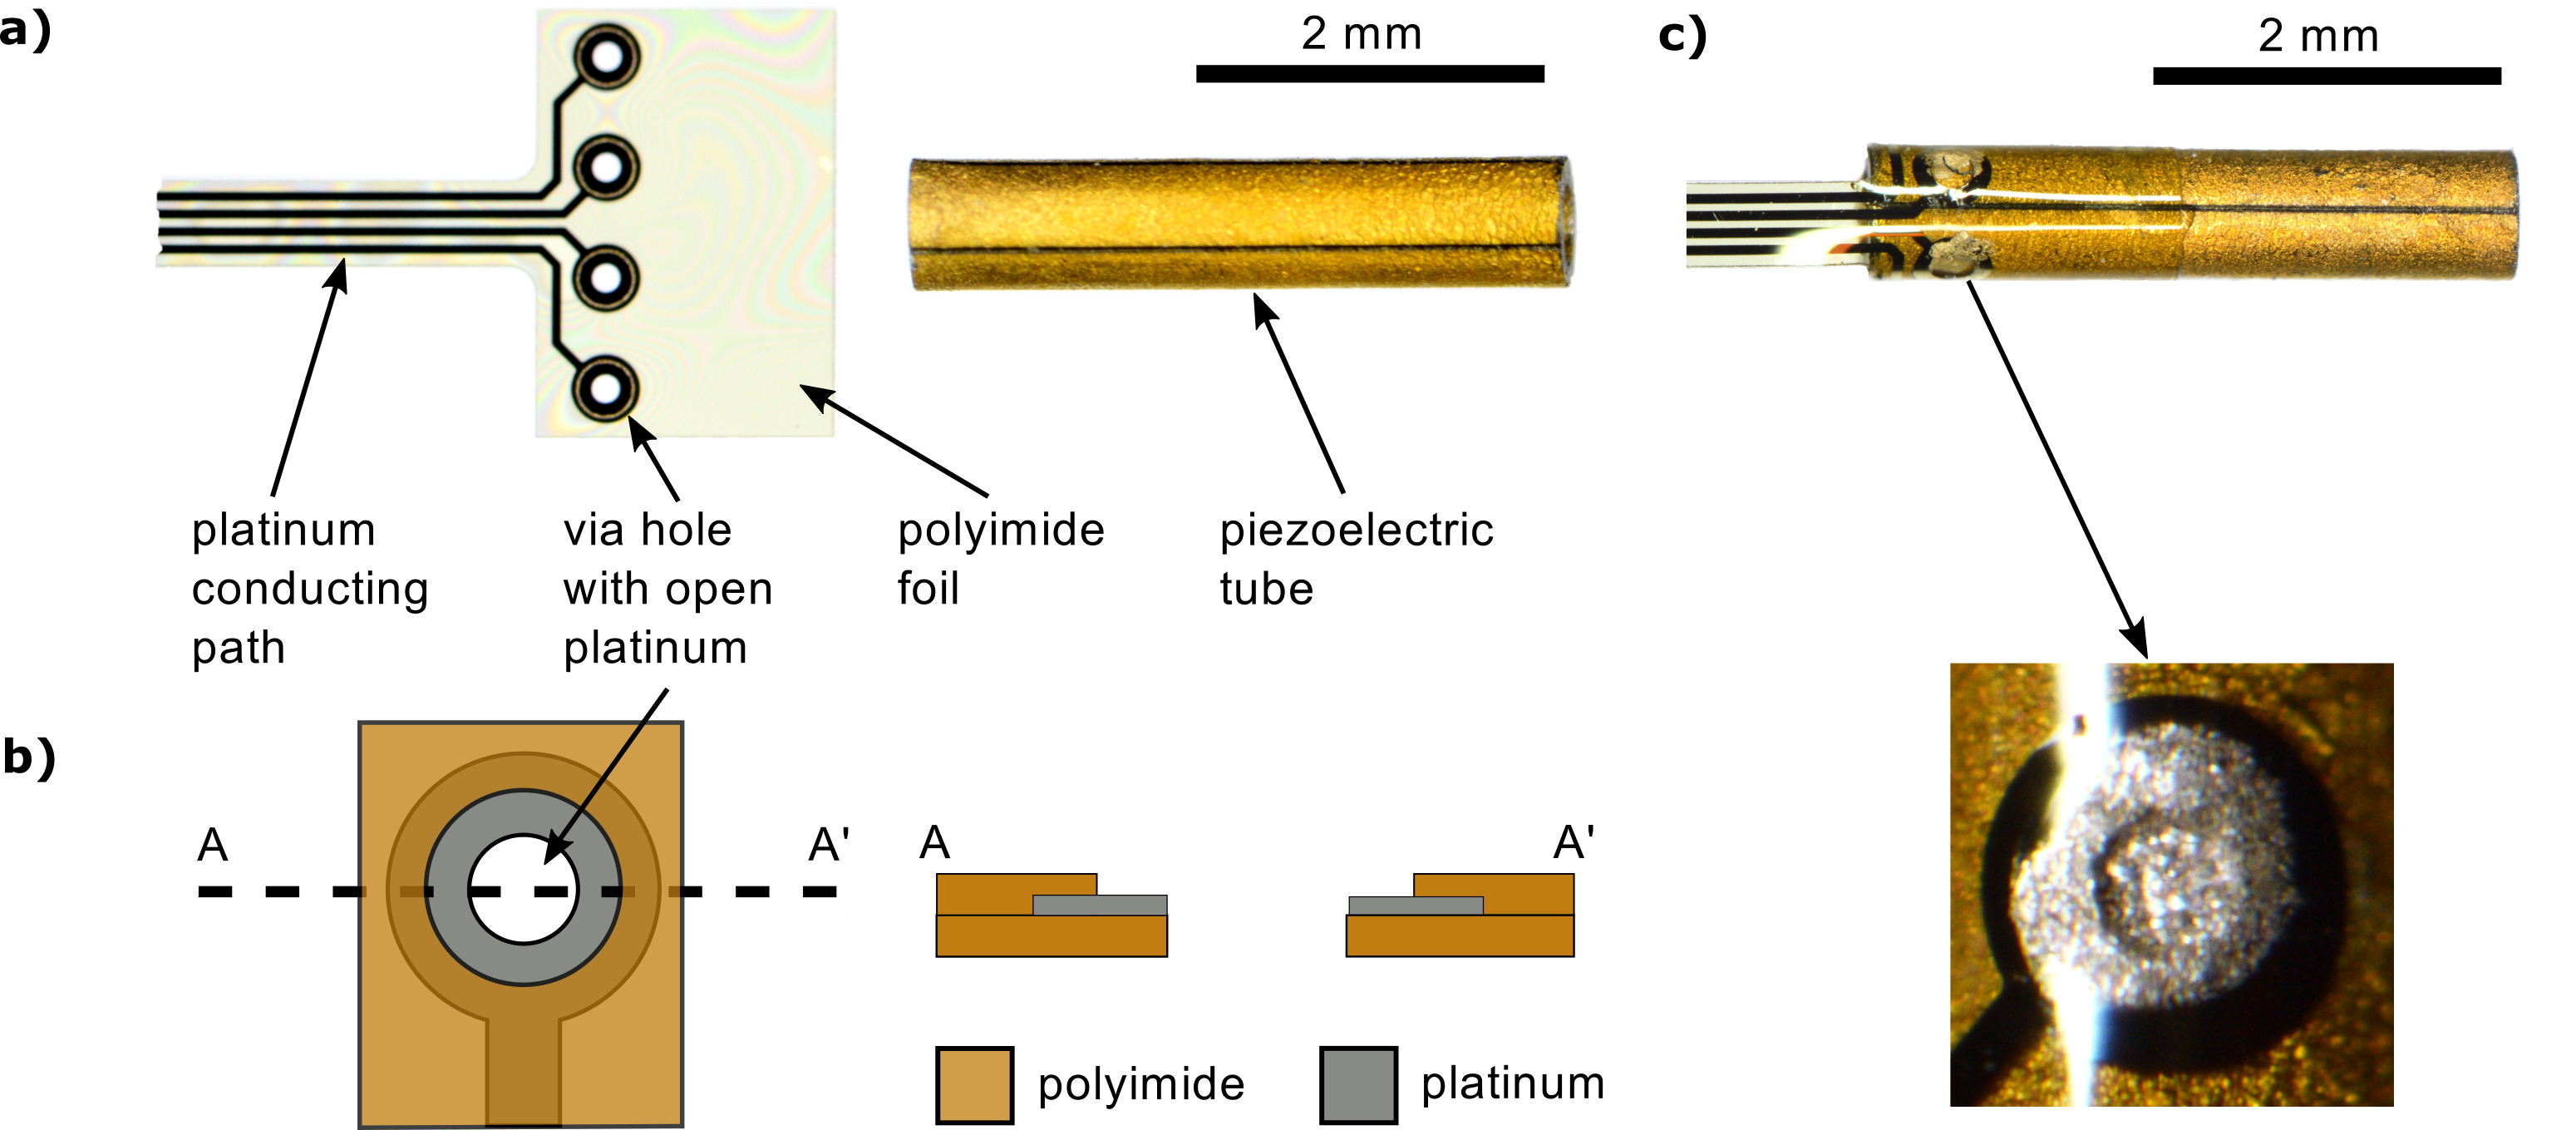
\includegraphics[width=\columnwidth]{figures/tubeFoilH.png}
      \caption{Polyimide electrode design.
      \textbf{a)} \textit{Left}: Photo of the polyimide ribbon cable with four vias to contact the four gold electrodes of the piezoelectric tube. \textit{Right}: Piezoelectric tube.
      \textbf{b)} Schematic of one via and its cross section. The platinum around the via is partly uncovered to improve the electrical connection between the cable and the piezoelctric tube.
      \textbf{c)} Photography of a polyimide ribbon cable, wrapped around the piezoelectric tube that is electrical connected through the vias by conductive glue.
      \textbf{d)} Microphotograph of the via after bonding with conductive glue, where a good wetting behavior can be observed.}
      \label{fig:piRolled}
\end{figure}

The polyimide ribbon cables are manufactured using a cleanroom process similar to the one developed for cuff electrodes for nerve stimulation \cite{Rodriguez2000} and consists of platinum tracks and via holes embedded in a polyimide substrate. One end the cable is shaped to fit a zero insertion force (ZIF) connector. The other end can be rolled around the piezoelectric tube, allowing the bonding to its gold electrodes using conductive glue (Araldite 2020 with 80\% wt. silver particles).

The polyimide ribbon cables are manufactured and singulated at wafer level. The process involves spin coating a \SI{5}{\micro\meter} layer of polyimide, which is cured at \SI{450}{\celsius} for \SI{10}{\minute}. Next, a \SI{100}{\nano\meter} layer of platinum is sputtered and patterned via liftoff, defining the conductive traces and the bondpads. On top of it, a second \SI{5}{\micro\meter} polyimide layer is spincoated and cured. Finally, the vias, openings and external shape of the cables are patterned through reactive ion etching (RIE), using the platinum as stop layer for the vias.

\begin{figure}[h!]\centering 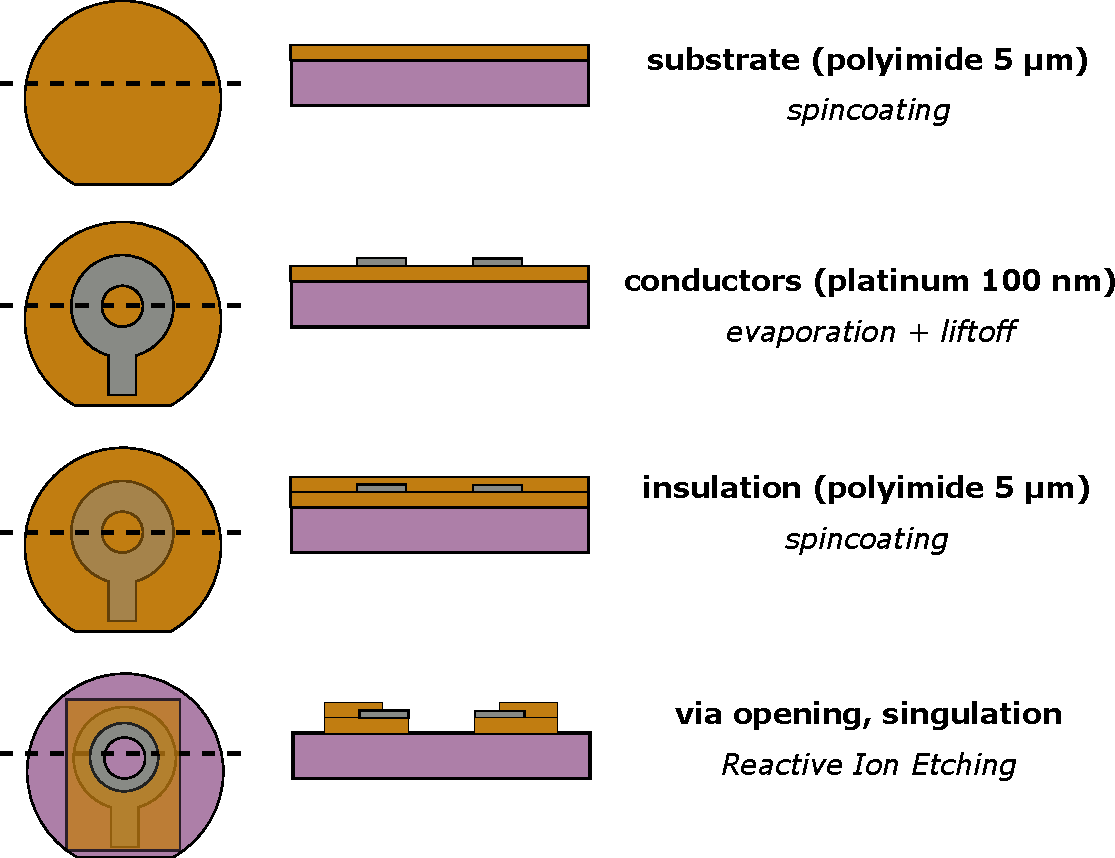
\includegraphics[width=\columnwidth]{figures/PIprocess.pdf}
      \caption{Polyimide electrodes}
      %\label{}
\end{figure}


\subsection{3D Printed housing}

The bimodal probe is designed to be assembled using the silicon bench technology \cite{Kretschmer}. But for the demonstrator, a process with reduced complexity, which allows faster design adjustments has been tested using a 3D printed polymer structure for both assembly and housing. This part was manufactured by B. Khatri (IMTEK) using a \textit{B9Creator} stereolithography printer, which allows the polimerization of an acrylic resin with a lateral resolution of \SI{30}{\micro\meter}.

This is possible because, even though the dimensional accuracy of the printed housing is lower than its silicon counterpart, the optical components of the demonstrator allow relatively high placement tolerances, as the beam is collimated in the region between GRIN lens and objective lens. This way, simple alignment structures which are 3D-printed within the housing allow the proper placement of all components, as shown in \autoref{fig:housing}. The main dimensions of the housing are depicted in \autoref{fig:housingDim}.


\begin{figure}[h!]\centering 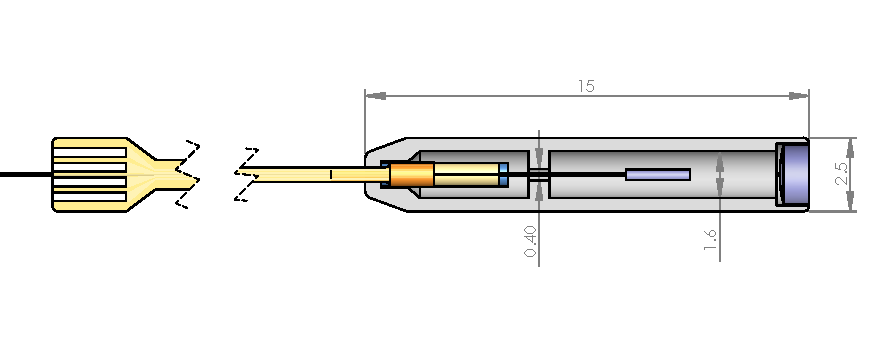
\includegraphics[width=\columnwidth]{figures/TopDrawing.pdf}
      \caption{Top view of the single modality probe showing the main dimensions of the housing.}
      \label{fig:housingDim}
\end{figure}

This relatively low resolution together with high part-to-part and batch-to-batch variations found in this method encourage a careful tolerance analysis during the design of the part. Nevertheless, these issues were compensated by the fast iterations in the design, allowing a successful implementation.


\subsection{Assembly}

Once all the components are ready, the assembly is performed manually using the multiple alignment features of the housing. The exploded view in \autoref{fig:exploded} shows the placement of the components prior to assembly, followed by the final encapsulation. This process is summarized as follows:

\begin{enumerate}
\item The GRIN lens is bonded to the end of the fiber using the alignment tool (\autoref{sec:fiberGRIN}).
\item The GRIN-fiber assembly is slid through the piezotube and centered with FR-2 fittings, which are glued to the piezotube using cyanocrilate.
\item The piezotube-fiber-GRIN assembly is placed in the bottom half of the housing and glued in place using cyanocrilate with help of the alignment structures.
\item The planoconvex lens is placed in the bottom half of the housing and glued using UV-curable optical glue.
\item The probe is closed with the top half of the housing and sealed with UV-curable glue.
\end{enumerate}

\begin{figure}[h!]\centering 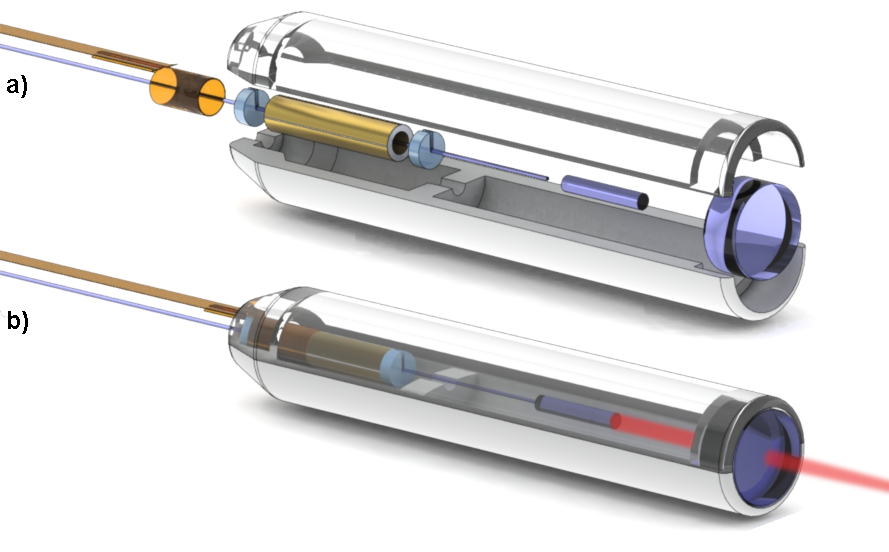
\includegraphics[width=\columnwidth]{figures/explodedRenderLaser.pdf}
      \caption{\textbf{a)} Exploded view of the components which form the single modality probe.
      \textbf{b)} Render of the complete probe after assembly.}
      \label{fig:exploded}
\end{figure}


%%%%%%%%%%%%%%%%%%%%%%%%%%%%%%%%%%%%%%%%%%%%%%%%%%%%%%%%%%%%%%%%%%%%%%%%
\section{Experimental evaluation}
%%%%%%%%%%%%%%%%%%%%%%%%%%%%%%%%%%%%%%%%%%%%%%%%%%%%%%%%%%%%%%%%%%%%%%%%

\subsection{Dynamic behavior of the scanner}
\label{sec:whirling}
The use of fiber scanners for imaging involves the challenge of whirling, identified already in the first fiber scanner implementations \cite{Seibel2001}.

This effect can be explained as follows: If a cantilever is rotationally symmetric, it will exhibit a single transversal resonant frequency. In this case, according to linear theory, if the base is excited in only one plane, the fiber will also only vibrate in that plane. But if a cantilever shows a small misalignment or non symmetric cross section -- as expected in any real world implementation -- it will exhibit two different frequency responses with peaks $f_x$ and $f_y$, corresponding to two planes of symmetry or eigendirections $x,y$, as can be seen in the example from \autoref{fig:bode}a. Far away from resonance the difference between axes is minimal. But close to resonance, these nonlinear effects create a cross-plane instability in which excitation of the base of the resonator in the $x$ direction can lead to oscillations in both $x$ and $y$ directions. This effect can be seen in the whirl plots of \autoref{fig:bode}b. 

\begin{figure}[h!]\centering 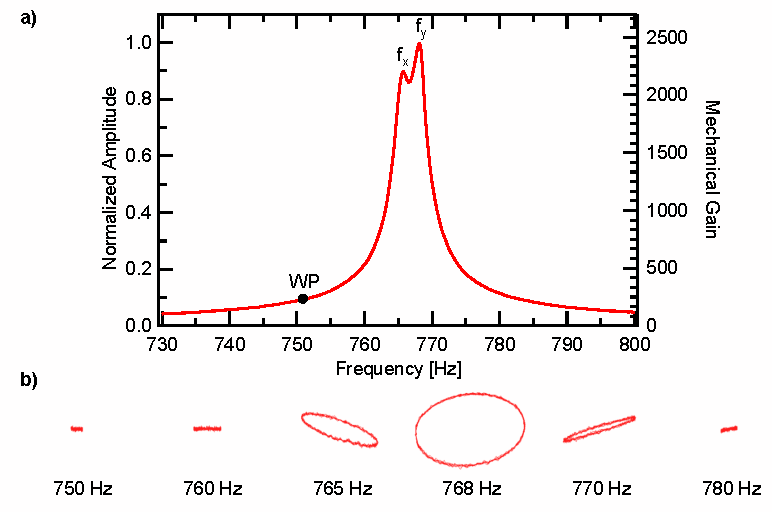
\includegraphics[width=\columnwidth]{figures/bodeWhirl.pdf}
      \caption{\textbf{a)} Dynamic behavior of the scanner in \textit{Probe 2} under harmonic excitation. The two eigenfrequencies corresponding to the main axes of the scanner are marked as $f_\mathrm{x} = \SI{765.8}{\hertz}$ and $f_\mathrm{y} = \SI{768.1}{\hertz}$.
      The Working Point WP shows a gain of 220. 
      The right axis shows the mechanical gain due to resonance, defined as the ratio of the displacement of the GRIN tip to the displacement of the piezoelectric tube tip.
      \textbf{b)} Whirl patterns obtained by exciting the scanner in the $x$ direction with different harmonic frequencies while measuring the position of the fiber tip. }
      \label{fig:bode}
\end{figure}

Therefore, for the imaging experiments, the scanner operates at a working point \textit{WP} far away from the resonance, in order to minimize the effect of whirling, but with a gain high enough to achieve the required amplitude of oscillation.


\subsection{Laser scanning imaging}
This section explains how it is possible to use the single modality probe for laser scanning imaging (LSI) and use the acquired images to assess its lateral resolution and depth of field. As OCT uses the concept of LSI to recreate volumetric images, these results are also representative for OCT imaging.

\subsection{Imaging}
The setup used to measure the backreflectivity of the probe, shown in \autoref{fig:confSetup}, can be used directly for LSI. While the probe scans an object with a spiral pattern defined by the driving voltage datapoints $(\mathbf{u_x}[n], \mathbf{u_y}[n])$, the data acquisition system (DAQ) samples a stream of intensities at the photodetector $\mathbf{I}[n]$, as shown in \autoref{fig:confPlotting}a. As these signals are generated and acquired synchronously, we expect that the intensity $\mathbf{I}[i]$ corresponds to a point in object space linearly related to the driving voltage of the piezoelectric scanner: $(x, y) = K_\mathrm{mech}(\mathbf{u_x}[i], \mathbf{u_y}[i])$, where $K_\mathrm{mech}$ is a mechanical constant.

\begin{figure}[h!]\centering 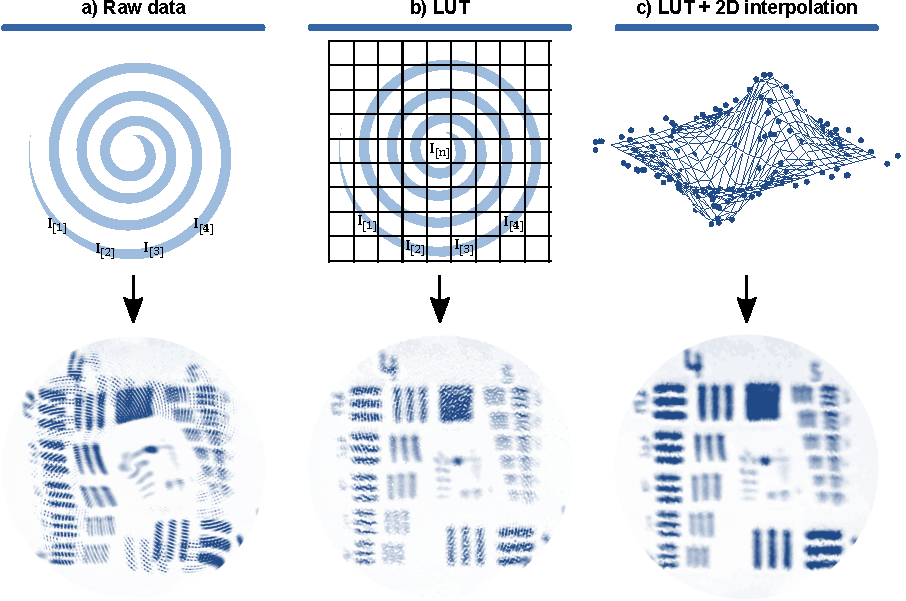
\includegraphics[width=\columnwidth]{figures/Plotting.pdf}
      \caption{Different representations of the same acquired datapoints $\mathbf{I}[n]$ of a USAF 1951 resolution test chart. The full acquired spiral consists of 374 rings of 122 datapoints, adding up to 45500 datapoints measured at \SI{91}{\kilo\hertz} during \SI{500}{\milli\second}. The field of view is \SI{1.1}{\milli\meter}.
      \textbf{a}: Point cloud assuming ideal movement of the scanner.
      \textbf{b}: Point cloud after correcting the position of each dot using a lookup table.
      \textbf{c}: Raster image after performing a 2D interpolation from the data in d.}
      \label{fig:confPlotting}
\end{figure}

If all the datapoints $\mathbf{I}_{[n]}$ acquired during a full spiral are plotted as a intensity-coded dot located at the position $K_\mathrm{mech}(\mathbf{u_x}[n], \mathbf{u_y}[n])$, the resultant image would look as in \autoref{fig:confPlotting}a: distorted. Notice how the dot plot defines two overlaid whirling images. This proves that the previous assumption of linearity is not valid, and thus the relationship between $(\mathbf{u_x}[i], \mathbf{u_y}[i])$ and $(\mathbf{x}[i], \mathbf{y}[i])$ is neither linear nor simple. This is the result of whirling, as discussed in \autoref{sec:whirling}. There are two general methods to overcome this problem:

The first one involves closed loop operation, where the current position of the scanner is measured inside the probe and used by the plotting system to correct for the distortion \cite{Yeoh2014}. 

The open loop alternative, used in this work, assumes that the distortion pattern is constant for a given driving signal. Then, the distorted spiral pattern $(x[i], y[i])$ can be measured after the assembly of the probe using a position sensitive device (PSD) and stored as a calibration lookup table.
Once this calibration step is performed, any further frame is plotted by assigning a position $(\mathbf{x}[i], \mathbf{y}[i])$ to every measured intensity $\mathbf{I}[n]$, as depicted in \autoref{fig:confPlotting}b, resulting in a distortionless dot plot. This procedure can be performed in real time.

The dot plots which are obtained from spiral scanners have the inconvenient of non-uniform sampling, as can be seen in \autoref{fig:calib}. Thus, to ease the further processing of the acquired images, it is beneficial to convert the non-uniform dot plot into a cartesian raster image. This can be performed by 2D interpolation, resulting in \autoref{fig:confPlotting}c.


\subsection{Lateral resolution measurement}
The optical performance of the scanner is qualitatively evaluated by capturing a SLI image of a USAF 1951 resolution test chart with a spiral scanning pattern using the setup described in \autoref{fig:confSetup}. As can be seen in \autoref{fig:confPlotting}c, element 4 of group 4 is resolved, indicating a resolution of 22 line pairs/mm or \SI{45}{\micro\meter}. 

A more robust method for the calculation of the optical resolution is detailed in \autoref{ssec:PSFMTF}: by manually scanning the focus of the probe over a sharp chromium edge of the test chart, the edge spread function (ESF) shown in \autoref{fig:MTF}a is obtained. By performing a spatial derivative followed by a Fourier transform of the ESF, the MTF can be obtained, plotted in \autoref{fig:MTF}b. Based on this curve the lateral resolution of the OCT beam path was determined at 21 line pairs/mm or \SI{47.6}{\micro\meter}. This value is very close to the theoretical resolution, calculated in \autoref{sec:ZEMAX} as 23.3 line pairs/mm or \SI{43}{\micro\meter}.
\begin{figure}[h!]\centering 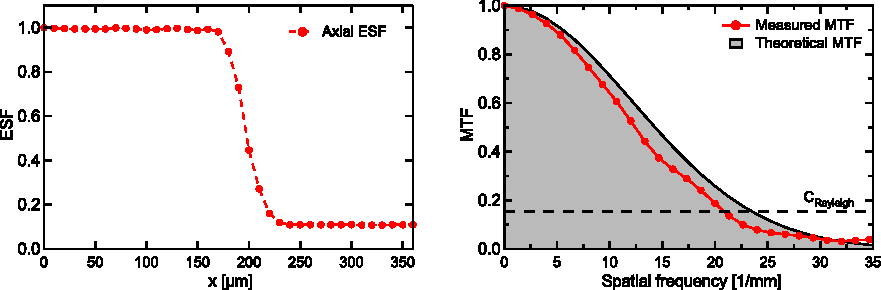
\includegraphics[width=\columnwidth]{figures/confResMeas.pdf}
      \caption{Left: Measured edge spread function (ESF) of the OCT beampath for the center of the field of view. 
      Right: Corresponding MTF compared with the theorical limit using the theory from \autoref{ssec:LSI}.}
      \label{fig:MTF}
\end{figure}
A good concordance is observed between the shape of the analytical and the measured MTF curves of the scanning modality. However, the overall performance is reduced by 10\% compared to the simulation. This deviation can be explained by small misalignments of the optical components induced by the process tolerances of the 3D-printed housing and the assembly process. Since a better alignment can be achieved in the silicon micro bench due to the higher precision of the MEMS processes a better match between simulation and reality can be expected for the multimodal probe.


\subsection{Depth of field measurement}
The depth of field (DOF) of the OCT imaging system can me determined by measuring how much light is backreflected upon a mirror while displacing it though the z axis. The results from this experiment are plotted in \autoref{fig:FWHM}, where a full width half maximum (FWHM) DOF of \SI{3.5}{\milli\meter} is calculated. 

\begin{figure}[h!]\centering 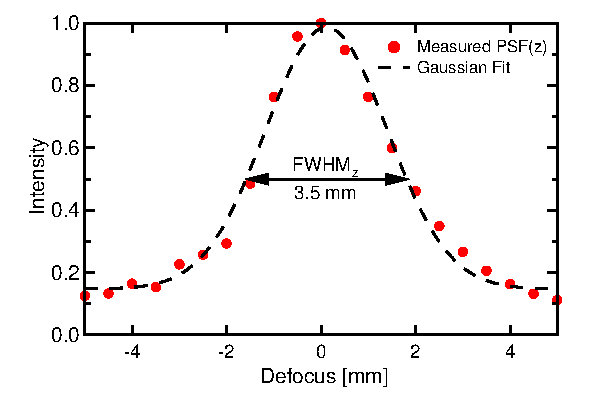
\includegraphics[width=\columnwidth]{figures/PSFz.pdf}
      \caption{Measurement of the axial resolution of the single modality probe. The intensity of the light coupled back into the optical system after reflection on a mirror is plotted against the manual translation of the mirror by $\pm \SI{4.5}{\milli\meter}$ from the focal plane of the probe. }
      \label{fig:FWHM}
\end{figure}




\subsection{OCT imaging}

The OCT characterization was performed using a swept-source OCT system property of the Medical University Vienna. This systemoperates with a center wavelength of \unit[1.34]{$\mu$ m}, a bandwidth of \unit[37]{nm} and a theoretical axial resolution in air of \unit[26.9]{$\mu$ m}.


The first OCT tests were performed as a proof of concept. Circular B-Scans of a colon polyp and a fingertip were captured with the single modality demonstrator, shown in \autoref{fig:B-Scan}. 
\begin{figure}[h!]\centering \includegraphics[width=\columnwidth]{figures/OCT_Measurement_arrangement}
      \caption{a) Illustration of the measurement arrangement for the circular B-Scan used as a proof of concept of OCT. b) Image of a circular OCT B-Scan of a colon polyp with a diameter $d=0.8\,\text{mm}$. Structural changes within the tissue can be detected and at the current state of the investigation the images suggest that blood vessels can be detected.
      c) Image of a circular OCT B-Scan of a human finger tip, where the epidermis, dermis and hypodermis can be tentatively differentiated.}
      \label{fig:B-Scan}
\end{figure}

These preliminary results prove that OCT imaging is possible. But at the same time, the low SNR of these images indicate that the designed system, which has a NA of 0.022, has problems collecting enough backscattered light. Therefore, future implementations of the probe could benefit from a higher NA. In that case, the resolution and collection of light of the system would be increased at the cost of a shorter working distance and a shorter depth of field. 



%%%%%%%%%%%%%%%%%%%%%%%%%%%%%%%%%%%%%%%%%%%%%%%%%%%%%%%%%%%%%%%%%%%%%%%%
\section{Discussion}
%%%%%%%%%%%%%%%%%%%%%%%%%%%%%%%%%%%%%%%%%%%%%%%%%%%%%%%%%%%%%%%%%%%%%%%%

%%%%%%%%%%%%%%%%%%%%%%%%%%%%%%%%%%%%%%%%%%%%%%%%%%%%%%%%%%%%%%%%%%%%%%%%
\section{Conclusion}
%%%%%%%%%%%%%%%%%%%%%%%%%%%%%%%%%%%%%%%%%%%%%%%%%%%%%%%%%%%%%%%%%%%%%%%%


%///////////////////////////////////////////////////////////////////////
%///////////////////////////////////////////////////////////////////////
\end{document}
%///////////////////////////////////////////////////////////////////////
%///////////////////////////////////////////////////////////////////////


This thesis realizes a novel fiber scanner in a telecentric configuration which reduce the distortion in the OCT modality and enables its integration within a multi-modal probe with dimensions of $13 \times 2 \times \SI{3}{\milli\meter^3}$. The complete scanning engine has an outer diameter of \SI{0.9}{\milli\meter} and a length of \SI{9}{\milli\meter}, and features custom fabricated \SI{10}{\micro\meter} thick polyimide flexible interconnect lines to address the four piezoelectric electrodes. The small cross section of the probe combined with its short length enables its use in a wide gamut of lumens in form of flexible or tilting head endoscope.

A single modality probe was designed to independently investigate the performance of the OCT beampath. This probe, depicted in \ref{fig:approachSketch}a, has an external diameter of \SI{2.5}{\milli\meter} and a total length of \SI{15}{\milli\meter}. Its optical design emulates that of the multimodal probe OCT path, enabling a direct translation of the results from this demonstrator probe to the multimodal one. To the best of our knowledge, this single modality probe is also one of the most compact implementation of an OCT microendoscope.

Using the demonstrator probe, it was possible to obtain preliminary \textit{en face} (\ref{fig:approachSketch}b) and tomographic (\ref{fig:approachSketch}c) images within a cylindrical volume of \SI{1}{\milli\meter} diameter and \SI{3}{\milli\meter} depth.

\section{Requirements}
\paragraph{Mechanical Requirements} 
\begin{itemize}

\item The scanner, electrical connections and optics should fit in a channel with a $\SI{1}{\milli\meter} \times \SI{1}{\milli\meter}$ cross section located in the lower level of a multimodal bench. This way the total cross section of the endoscope can be kept below $3 \times \SI{2}{\milli\meter^2}$). 
\item Its length should be minimized to allow its integration in flexible-head endoscopes.
\item The field of view should be maximized for a 2 mm diameter objective lens that is shared with the endomicroscopy beam path.
\item The scanning speed should be adequate for the sampling rates characteristic of SS-OCT ($\sim \SI{100}{\kilo\hertz} $).
\end{itemize}


\paragraph{Optical Requirements}

\begin{itemize}
\item The microscopy and OCT imaging fields should be coaxial to allow the registration of both images. 
\item The OCT field should be telecentric to avoid field curvature distortions.
\item The lateral resolution and depth of field should be adequate for OCT i.e. with numerical aperture ranging from 0.02 to 0.05.
\item The backreflections inside the probe should be minimized to reduce any loss of contrast and penetration depth.
\end{itemize}








%%*****************************************************************************
\section{Image acquisition: spiral scanning}
\label{sec:spiralScanning}
%%*****************************************************************************



%%*****************************************************************************
\section{Mechanical design}
\label{sec:mechDesign}
%%*****************************************************************************

\section{Implementation}
\label{Ch:Fab}	






\section{Conclusion \& Outlook}

%The main goal of this work was the realization of a novel single-fiber-based scanning scheme enabling simultaneous 3D OCT in combination with full field microscopy using spectrally separated beampaths in a probe with dimensions of only $13 \times 2 \times \SI{3}{\milli\meter^3}$. 

The main goal of this work is the realization of a novel fiber scanner for 3D OCT imaging, designed for its combination with a full field microscope to form a multimodal probe. A tubular piezoelectric fiber scanner is used to perform en face scanning required for 3D OCT measurements. The complete scanning engine has an outer diameter of \SI{0.9}{\milli\meter} and a length of \SI{9}{\milli\meter}, and features custom fabricated \SI{10}{\micro\meter} thick polyimide flexible interconnect lines to address the four piezoelectric electrodes. This scanning engine was tested in a single modality, demonstrator probe with an external diameter of \SI{2.5}{\milli\meter} and a total length of \SI{15}{\milli\meter}, allowing the OCT imaging of a \SI{1}{\milli\meter} field of view with a resolution of \SI{45}{\micro\meter} using \SI{1330}{\nano\meter} light. 

To the best of our knowledge, the presented demonstrator probe is also one of the most compact implementation of an OCT microendoscope.

\section{Conclusion}
During this project, the behavior of fiber scanners was analyzed and several approaches were discussed and simulated. It was concluded that its implementation as fourier plane scanner using a GRIN lens as collimator and weight was optimal for OCT. A complete electro-mechano-optical analysis and simulation followed, allowing the optimization of the system to reach diffraction-limited resolution and a maximum field of view.

The size constraints that required the implementation of the scanner in a $1\times \SI{1}{\milli\meter^2}$ channel in the bottom of the bench challenged the electrical contacting of the \SI{800}{\micro\meter} diameter piezoelectric actuator. The solution involved the fabrication of a novel \SI{10}{\micro\meter} thick polyimide ribbon cable that can be rolled around the tube and contacted to it using vias and conductive glue. The cleanroom process proved to be reliable and repeatable, encouraging its use in upcoming projects.

This work also demonstrated the bonding of a single mode, \SI{80}{\micro\meter} optical fiber to a GRIN lens using a custom silicon microfabricated tool. This method allowed a placement accuracy in the \SI{}{\micro\meter} range, creating an optical and mechanical bond that operates reliably under the high mechanical stress found in a resonant scanner. Prior OCT setups including GRIN lenses showed that they can cause problematic backreflections. This problem was successfully avoided by a custom GRIN lens design with a \SI{1}{\degree} tilted exit facet. This solution, together with an special attention to the layout of the optical components, resulted in an optical system with backreflections below 0.02\%.

The assembly of the single mode demonstrator was successfully achieved using alignment features integrated in a 3D-printed housing. This part was manufactured using a commercial, low cost stereolithographic resin printer that enabled quick iterations of the design. The manufactured demonstrator allowed the analysis and proof of concept of the fiber scanner concept. Experimental measurements helped refining the assumptions used in the analytical calculation of the resolution of OCT systems. The resultant theoretical description, which closely matches experimental results, will help in the design of future OCT and confocal systems. Although previous work at IMTEK had proven the use of fiber scanners for confocal imaging \cite{Meinert}, further analysis was needed to understand and correct for the imaging distortions caused by whirling. The calibration method used in this work, which can operate in real time, reduces the imaging distortions to a minimum and enables the quantitative analysis of the acquired image. This enabled going one step further in cooperation with the Medical University Vienna, where the OCT imaging concept was proven, creating new opportunities for collaboration. 



